%package list
\documentclass{article}
\usepackage[top=3cm, bottom=3cm, outer=3cm, inner=3cm]{geometry}
\usepackage{multicol}
\usepackage{graphicx}
\usepackage{url}
%\usepackage{cite}
\usepackage{hyperref}
\usepackage{array}
%\usepackage{multicol}
\newcolumntype{x}[1]{>{\centering\arraybackslash\hspace{0pt}}p{#1}}
\usepackage{natbib}
\usepackage{pdfpages}
\usepackage{multirow}
\usepackage[normalem]{ulem}
\useunder{\uline}{\ul}{}
\usepackage{svg}
\usepackage{xcolor}
\usepackage{listings}
\lstdefinestyle{ascii-tree}{
    literate={├}{|}1 {─}{--}1 {└}{+}1 
  }
\lstset{basicstyle=\ttfamily,
  showstringspaces=false,
  commentstyle=\color{red},
  keywordstyle=\color{blue}
}
%\usepackage{booktabs}
\usepackage{caption}
\usepackage{subcaption}
\usepackage{float}
\usepackage{array}

\newcolumntype{M}[1]{>{\centering\arraybackslash}m{#1}}
\newcolumntype{N}{@{}m{0pt}@{}}


%%%%%%%%%%%%%%%%%%%%%%%%%%%%%%%%%%%%%%%%%%%%%%%%%%%%%%%%%%%%%%%%%%%%%%%%%%%%
%%%%%%%%%%%%%%%%%%%%%%%%%%%%%%%%%%%%%%%%%%%%%%%%%%%%%%%%%%%%%%%%%%%%%%%%%%%%
\newcommand{\itemEmail}{rcompanocca@unsa.edu.pe}
\newcommand{\itemStudent}{Roni Companocca Checco}
\newcommand{\itemCourse}{Programación}
\newcommand{\itemCourseCode}{20210558}
\newcommand{\itemSemester}{II}
\newcommand{\itemUniversity}{Universidad Nacional de San Agustín de Arequipa}
\newcommand{\itemFaculty}{Facultad de Ingeniería de Producción y Servicios}
\newcommand{\itemDepartment}{Departamento Académico de Ingeniería de Sistemas e Informática}
\newcommand{\itemSchool}{Escuela Profesional de Ingeniería de Sistemas}
\newcommand{\itemAcademic}{2023 - B}
\newcommand{\itemInput}{Del 28 octubre 2023}
\newcommand{\itemOutput}{Al 2 Noviembre 2023}
\newcommand{\itemPracticeNumber}{12}
\newcommand{\itemTheme}{Definición de Clases de Usuario Clase Soldado - Menú}
%%%%%%%%%%%%%%%%%%%%%%%%%%%%%%%%%%%%%%%%%%%%%%%%%%%%%%%%%%%%%%%%%%%%%%%%%%%%
%%%%%%%%%%%%%%%%%%%%%%%%%%%%%%%%%%%%%%%%%%%%%%%%%%%%%%%%%%%%%%%%%%%%%%%%%%%%

\usepackage[english,spanish]{babel}
\usepackage[utf8]{inputenc}
\AtBeginDocument{\selectlanguage{spanish}}
\renewcommand{\figurename}{Figura}
\renewcommand{\refname}{Referencias}
\renewcommand{\tablename}{Tabla} %esto no funciona cuando se usa babel
\AtBeginDocument{%
	\renewcommand\tablename{Tabla}
}

\usepackage{fancyhdr}
\pagestyle{fancy}
\fancyhf{}
\setlength{\headheight}{30pt}
\renewcommand{\headrulewidth}{1pt}
\renewcommand{\footrulewidth}{1pt}
\fancyhead[L]{\raisebox{-0.2\height}{
\includegraphics[width=3cm]{logo_episunsa.png}}}
\fancyhead[C]{\fontsize{7}{7}\selectfont	\itemUniversity \\ \itemFaculty \\ \itemDepartment \\ \itemSchool \\ \textbf{\itemCourse}}
\fancyhead[R]{\raisebox{-0.2\height}{
\includegraphics[width=1.2cm]{abet.png}}}
\fancyfoot[L]{Estudiante Roni Companocca Checco}
\fancyfoot[C]{\itemCourse}
\fancyfoot[R]{Página \thepage}

% para el codigo fuente
\usepackage{listings}
\usepackage{color, colortbl}
\definecolor{dkgreen}{rgb}{0,0.6,0}
\definecolor{gray}{rgb}{0.5,0.5,0.5}
\definecolor{mauve}{rgb}{0.58,0,0.82}
\definecolor{codebackground}{rgb}{0.95, 0.95, 0.92}
\definecolor{tablebackground}{rgb}{0.8, 0, 0}

\lstset{frame=tb,
	language=bash,
	aboveskip=3mm,
	belowskip=3mm,
	showstringspaces=false,
	columns=flexible,
	basicstyle={\small\ttfamily},
	numbers=none,
	numberstyle=\tiny\color{gray},
	keywordstyle=\color{blue},
	commentstyle=\color{dkgreen},
	stringstyle=\color{mauve},
	breaklines=true,
	breakatwhitespace=true,
	tabsize=3,
	backgroundcolor= \color{codebackground},
}

\begin{document}
	
	\vspace*{10px}
	
	\begin{center}	
		\fontsize{17}{17} \textbf{ Informe de Laboratorio \itemPracticeNumber}
	\end{center}
	\centerline{\textbf{\Large Tema: \itemTheme}}
	%\vspace*{0.5cm}	

	\begin{flushright}
		\begin{tabular}{|M{2.5cm}|N|}
			\hline 
			\rowcolor{tablebackground}
			\color{white} \textbf{Nota}  \\
			\hline 
			     \\[30pt]
			\hline 			
		\end{tabular}
	\end{flushright}	

	\begin{table}[H]
		\begin{tabular}{|x{4.7cm}|x{4.8cm}|x{4.8cm}|}
			\hline 
			\rowcolor{tablebackground}
			\color{white} \textbf{Estudiante} & \color{white}\textbf{Escuela}  & \color{white}\textbf{Asignatura}   \\
			\hline 
			{\itemStudent \par \itemEmail} & \itemSchool & {\itemCourse \par Semestre: \itemSemester \par Código: \itemCourseCode}     \\
			\hline 			
		\end{tabular}
	\end{table}		
	
	\begin{table}[H]
		\begin{tabular}{|x{4.7cm}|x{4.8cm}|x{4.8cm}|}
			\hline 
			\rowcolor{tablebackground}
			\color{white}\textbf{Laboratorio} & \color{white}\textbf{Tema}  & \color{white}\textbf{Duración}   \\
			\hline 
			\itemPracticeNumber & \itemTheme & 04 horas   \\
			\hline 
		\end{tabular}
	\end{table}
	
	\begin{table}[H]
		\begin{tabular}{|x{4.7cm}|x{4.8cm}|x{4.8cm}|}
			\hline 
			\rowcolor{tablebackground}
			\color{white}\textbf{Semestre académico} & \color{white}\textbf{Fecha de inicio}  & \color{white}\textbf{Fecha de entrega}   \\
			\hline 
			\itemAcademic & \itemInput &  \itemOutput  \\
			\hline 
		\end{tabular}
	\end{table}

    \section{TAREA}
	\begin{itemize}	
    \subsection{Objetivos:}
		\item Que el alumno demuestre poder crear  “clases definidas por el programador” 
		\item Implementar métodos para las clases definidas por el programador
       
    \subsection{Competencias a alcanzar:}
		\item Diseña, responsablemente, sistemas, componentes o procesos para satisfacer necesidades dentro de restricciones realistas: económicas, medio ambientales, sociales, políticas, éticas, de salud, de seguridad, manufacturación y sostenibilidad.
        \item Aplica de forma flexible, técnicas, métodos, principios, normas, estándares y herramientas de ingeniería necesarias para la construcción de software e implementación de sistemas de información.
    \subsection{Marco teorico:}
        \item Clase: Una Fábrica de objetos. Una clase está conformada por dos partes: datos miembro (variables de instancia / atributos) y los métodos. 
        \item Los métodos nos permiten acceder y/o modificar los datos miembros (atributos) de los objetos. 
        \item Toda clase necesita al menos un Constructor. El constructor lleva el mismo nombre de la clase. El constructor es un método especial que siempre se llama con la palabra reservada new() 
        
    \subsection{Indicaciones generales:}
        \item Todos los ejercicios deberán ser guardados en el mismo Proyecto
        \item El Proyecto deberá tener el nombre del Laboratorio y el nombre del alumno, así por ejemplo: Laboratorio 1 – Juan Perez
        \item Cada Clase deberá tener el nombre del ejercicio, así por ejemplo: Ejercicio1
        \item Utilice nombres de variables significativos y todas las recomendaciones de estilo
        \item Especialmente, su código deberá estar correctamente indentado
        \item Deberá pasar TODOS los casos de prueba
	\end{itemize}

    \section{EQUIPOS, MATERIALES Y TEMAS UTILIZADOS}
	\begin{itemize}
		\item Sistema Operativo Windows
		\item OpenJDK 64-Bits 17.0.7.
		\item Git 2.39.2.	
  	\item Cuenta en GitHub con el correo institucional.
	\end{itemize}

    \section{URL DE REPOSITORIO GITHUB}
	\begin{itemize}
		\item URL para el Repositorio GitHub.
		\item \url{https://github.com/RONI-COMPANOCCA-CHECCO}
		\item URL para el laboratorio 12 en el Repositorio GitHub.	
        \item \url{https://github.com/RONI-COMPANOCCA-CHECCO/FP2-LAB12}
	\end{itemize}
    
    \section{EJERCICIO PROPUESTO}
	\begin{itemize}

        \subsection{INTRODUCCION}
        \subsubsection {Este laboratorio requiere que usted escriba un programa utilizando clases definidas por el programador. No deberá utilizar sintaxis o constructores que no han sido cubiertos durante las clases teóricas. Será penalizado por esta falta. A menos que una plantilla sea dada, deberá utilizar cada programa desde cero de manera que obtenga suficiente práctica en la escritura de programas en Java.}
        \subsubsection Un consejo: Programe incrementalmente. No trate de terminar todas las partes del programa y luego compilarlo. Escriba sus programas en partes y compílelo de forma frecuente. Trate de mantener un programa compilable aun cuando esté trabajando en él. Presentar un programa compilable que funcione parcialmente es mejor que presentar un programa no-compilable.  EN SERIO, programe incrementalmente. 
        \item Los objetivos de este laboratorio son:
        \item Deberá asumir que todos los datos de ingreso son correctos. 
        \item Deberá utilizar la clase Scanner en System.in para ingresos de datos y System.out para salida de datos en sus programas, a menos que se indique lo contrario.
        \item Pruebe sus programas con sus propios datos de prueba antes de presentarlos. 
        \item Evitar duplicación de código.
        \item Usar como base el diagrama de clases UML siguiente (puede aumentar atributos y métodos necesarios):
        \item .
        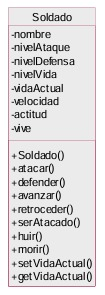
\includegraphics[height=10cm]{dia.jpeg}
        \item Puede reutilizar todo el código del laboratorio 11, pero ahora el objetivo es gestionar los ejércitos autogenerados. 
        \item Al ejecutar el videojuego, el programa deberá dar las opciones: 
        \paragraph 1. Juego rápido (tal cual como en el laboratorio 11) Al acabar el juego mostrar las opciones de volver a jugar y de volver al menú principal. También se deberá tener la posibilidad de cancelar el juego actual en cualquier momento, permitiendo escoger entre empezar un juego totalmente nuevo o salir al menú principal. 
        \paragraph 2. Juego personalizado: permite gestionar ejércitos. Primero se generan los 2 ejércitos con sus respectivos soldados y se muestran sus datos. Luego se tendrá que escoger cuál de los 2 ejércitos se va a gestionar, después se mostrarán las siguientes opciones: 
            \subparagraph 2.1 Crear Soldado: permitirá crear un nuevo soldado personalizado y añadir al final del ejército (recordar que límite es de 10 soldados por ejército)
        \item 2) Eliminar Soldado (no debe permitir un ejército vacío) 
        \item 3) Clonar Soldado (crea una copia exacta del soldado) y se añade al final del ejército (recordar que límite es de 10 soldados por ejército) 
        \item 4) Modificar Soldado (con submenú para cambiar alguno de los atributos nivelAtaque, nivelDefensa, vidaActual) 
        \item 5) Comparar Soldados (verifica si atributos: nombre, nivelAtaque, nivelDefensa, vidaActual y vive son iguales) 
        \item 6) Intercambiar Soldados (intercambia 2 soldados en sus posiciones en la estructura de datos del ejército) 
        \item 7) Ver soldado (Búsqueda por nombre) 
        \item 8) Ver ejército 
        \item 9) Sumar niveles (usando Method-Call Chaining), calcular las sumatorias de nivelVida, nivelAtaque, nivelDefensa, velocidad de todos los soldados de un ejército 
        \item 10) Jugar (se empezará el juego con los cambios realizados) y con las mismas opciones de la opción 1. 
        \item 11) Volver (muestra el menú principal) Después de escoger alguna de las opciones 1) a 9) se podrá volver a elegir uno de los ejércitos y se mostrarán las opciones 1) a 11) 
        \item 3. Salir 
        
        \begin{lstlisting}[language=java]
        // RONI COMPANOCCA CHECCO
// CUI: 20210558
// LABORATORIO 04
// FUNDAMENTOS DE PROGRAMACION 

        \end{lstlisting}

        \item la clase Nave.java
        \begin{lstlisting}[language=java]

         \end{lstlisting}
    
	\end{itemize}
	
	\section{REFERENCIAS}
	\begin{itemize}
		\item M. Aedo, “Fundamentos de Programación 2 - Tópicos de Programación Orientada a Objetos”, Primera Edición, 2021, Editorial UNSA.
		\item \url{https://github.com/rescobedoq/programacion.git}
		\item J. Dean, "Introduction to programming with Java: A Problem Solving Approach”, Third Edition, 2021, McGraw-Hill.
        \item C. T. Wu, "An Introduction to Object-Oriented Programming with Java", Fifth Edition, 2010, McGraw-Hill.
        \item P. Deitel, "Java How to Program", Eleventh Edition, 2017, Prentice Hall.
	\end{itemize}
	
%\clearpage
%\bibliographystyle{apalike}
%\bibliographystyle{IEEEtranN}
%\bibliography{bibliography}
			
\end{document}